
\section{Robustness Checks}

In our applications we have worked with a holding period of $L=4$ trading days and an upper bound on traded clusters of $\theta=\integer{0.5k}$. As shown in section A.2 of the Appendix, such choices result from the maximization of the Sharpe Ratios in the train and validation samples. All that is left is to check whether our out-of-sample results are sensitive to the choice of hyperparameters ($L,\theta$). For this purpose, we evaluate the variability of the Sharpe Ratios of the test portfolio ($SR^{\mathcal P^{test}}$) to changes in $L$ and $\theta$. 

\bx 
First, we focus on the holding period length of the beta-neutral strategy ($L$). For this purpose, we fix $\theta=\integer{0.5k}$ and, for each clustering method, obtain the series of Sharpe Ratios over a grid $\mbf L$ (which ranges from 1 to 20 trading periods). This delivers the series $\{SR^{\mathcal P ^{test}} (L)\}_{L\in\mbf L}$, which we then plot in two formats. On the left side of \cref{fig:LLM_Robustness_L} we plot the distribution of Sharpe Ratios in the grid, and in the right side, we show the mapping $L\mapsto SR^{\mathcal P ^{test}} (L)$ over $\mbf L$. 

%----------------------------------------------------
\inserthere{fig:LLM_Robustness_L}
\begin{figure}[H]
  \centering
  \caption{Sensitivity of $SR^{\mathcal P^{test}}$ to the holding window length ($L$)}
    \begin{subfigure}[b]{0.44\textwidth}
    \centering
    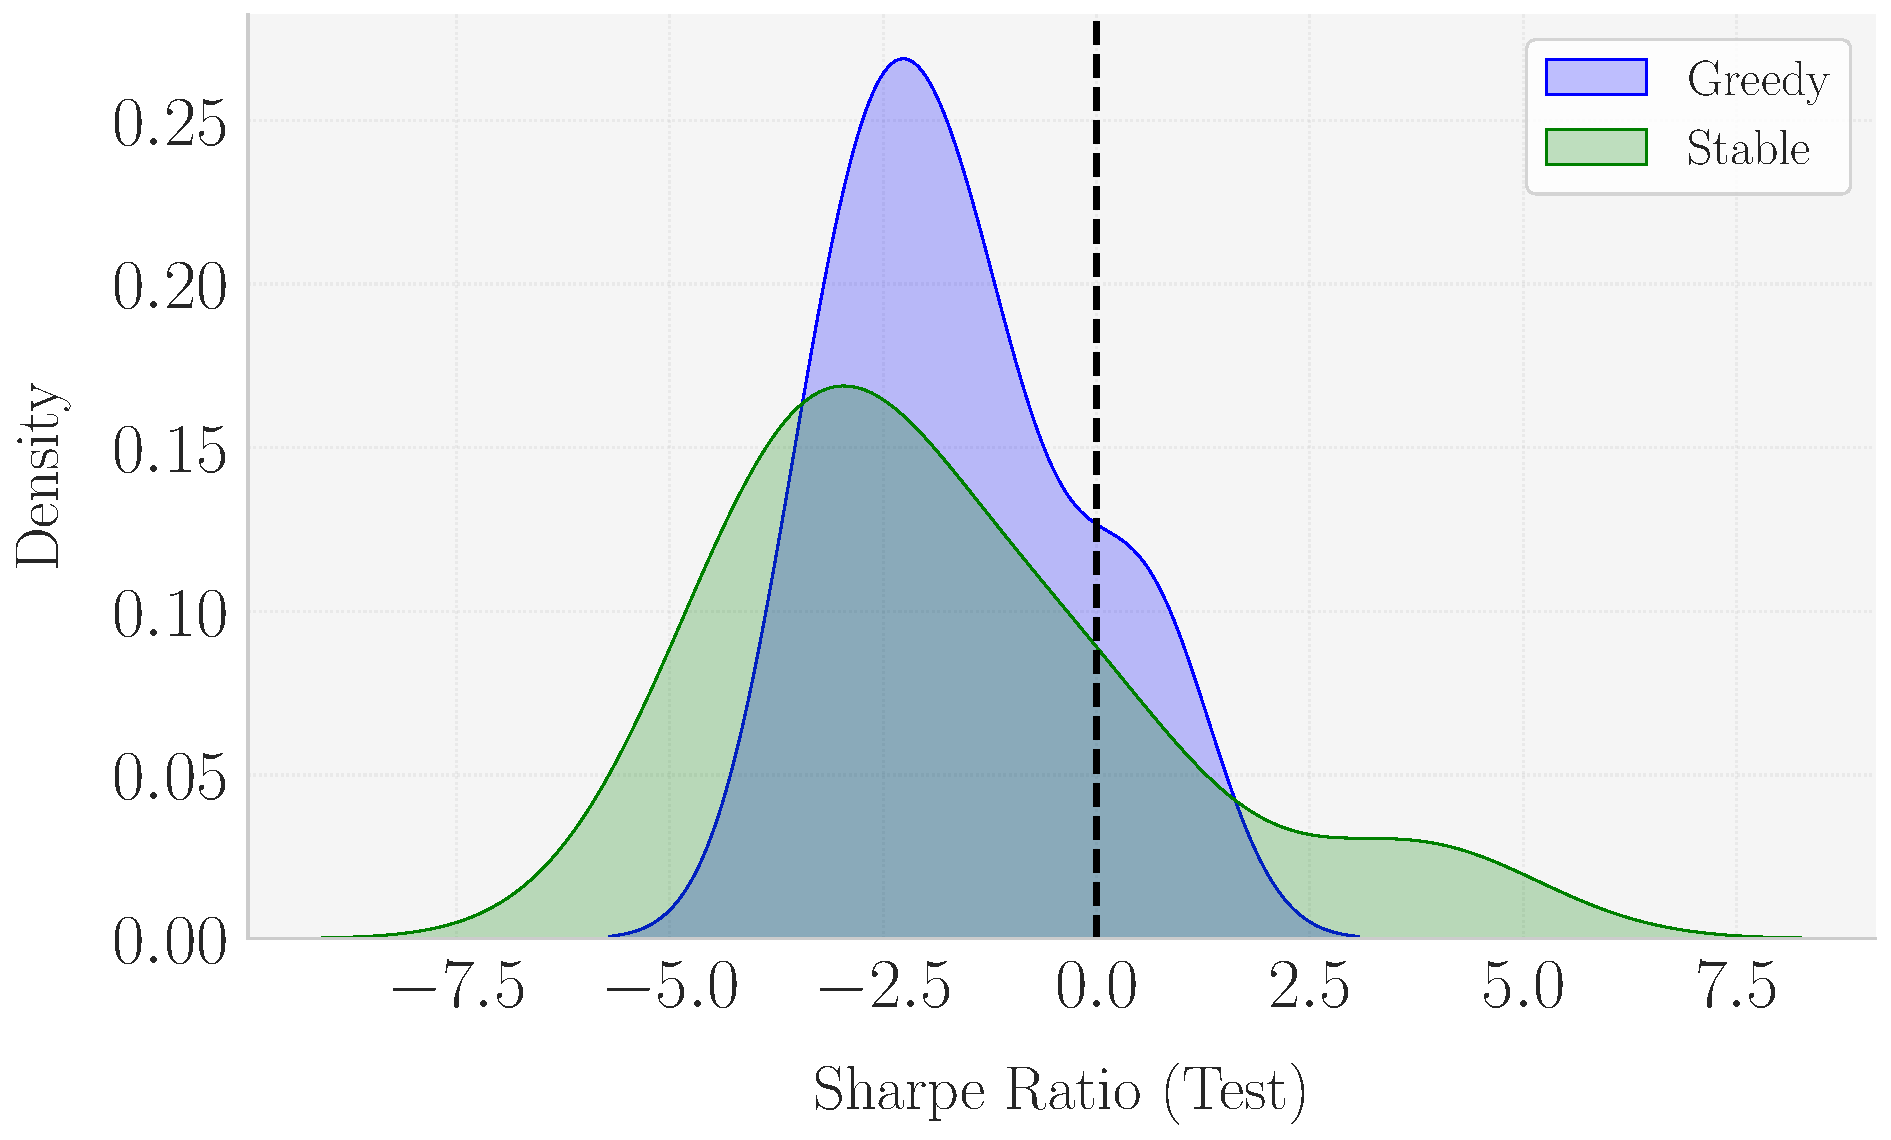
\includegraphics[width=\textwidth]{fig_8a_KMeans_RobustnessCheck_SR_Test_Set_Distribution_[Change_L].pdf}
    \caption{\textbf{KMeans}: Distribution of $SR^{\mathcal P^{test}}(L)$}
    \label{fig:KMeans_Robustness_L_Distr}
  \end{subfigure}
  \hspace{0.05\textwidth} % Add horizontal space between the subfigures
  \begin{subfigure}[b]{0.44\textwidth}
    \centering
    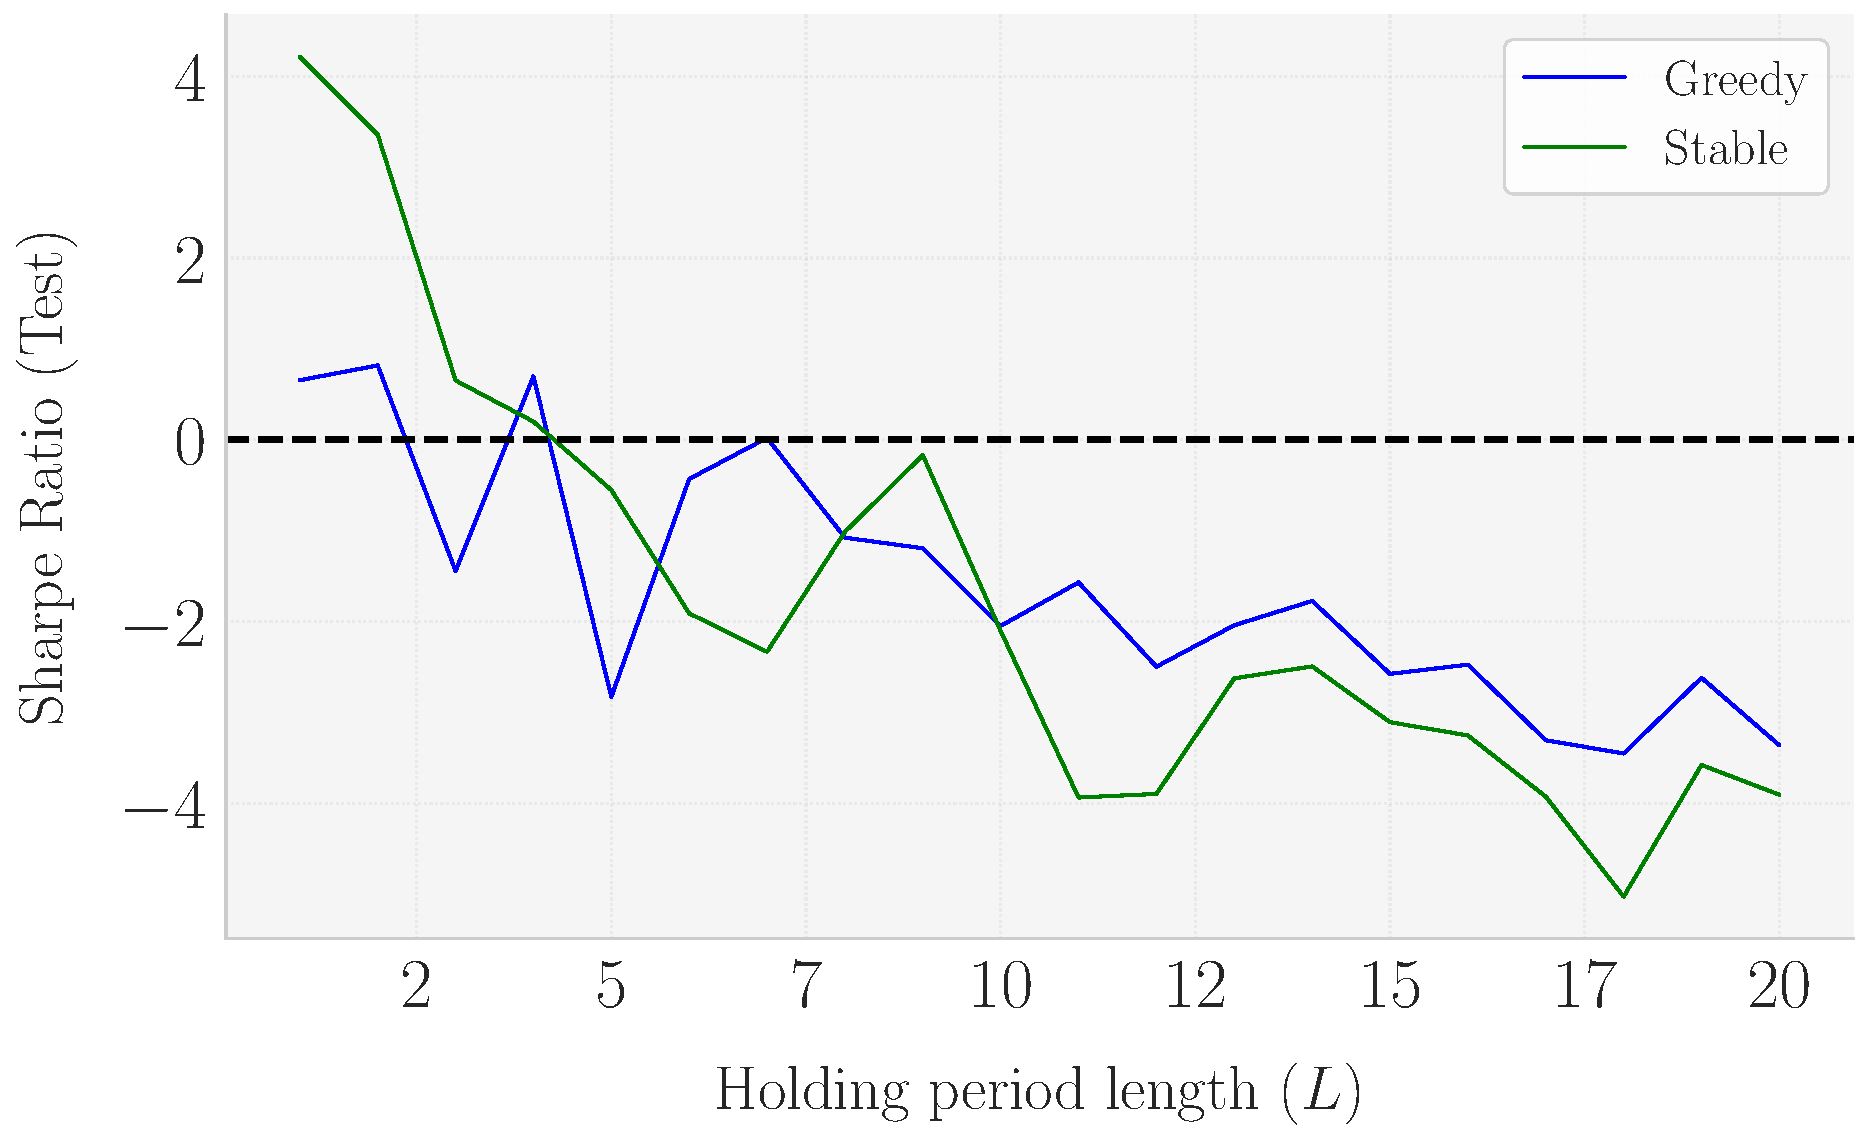
\includegraphics[width=\textwidth]{fig_8b_KMeans_RobustnessCheck_SR_Test_Set_vs_L_[Change_L].pdf}
    \caption{\textbf{KMeans}: Series of $SR^{\mathcal P^{test}}(L)$}
    \label{fig:KMeans_Robustness_L_Series}
  \end{subfigure}
  
  \bx 
      \begin{subfigure}[b]{0.44\textwidth}
    \centering
    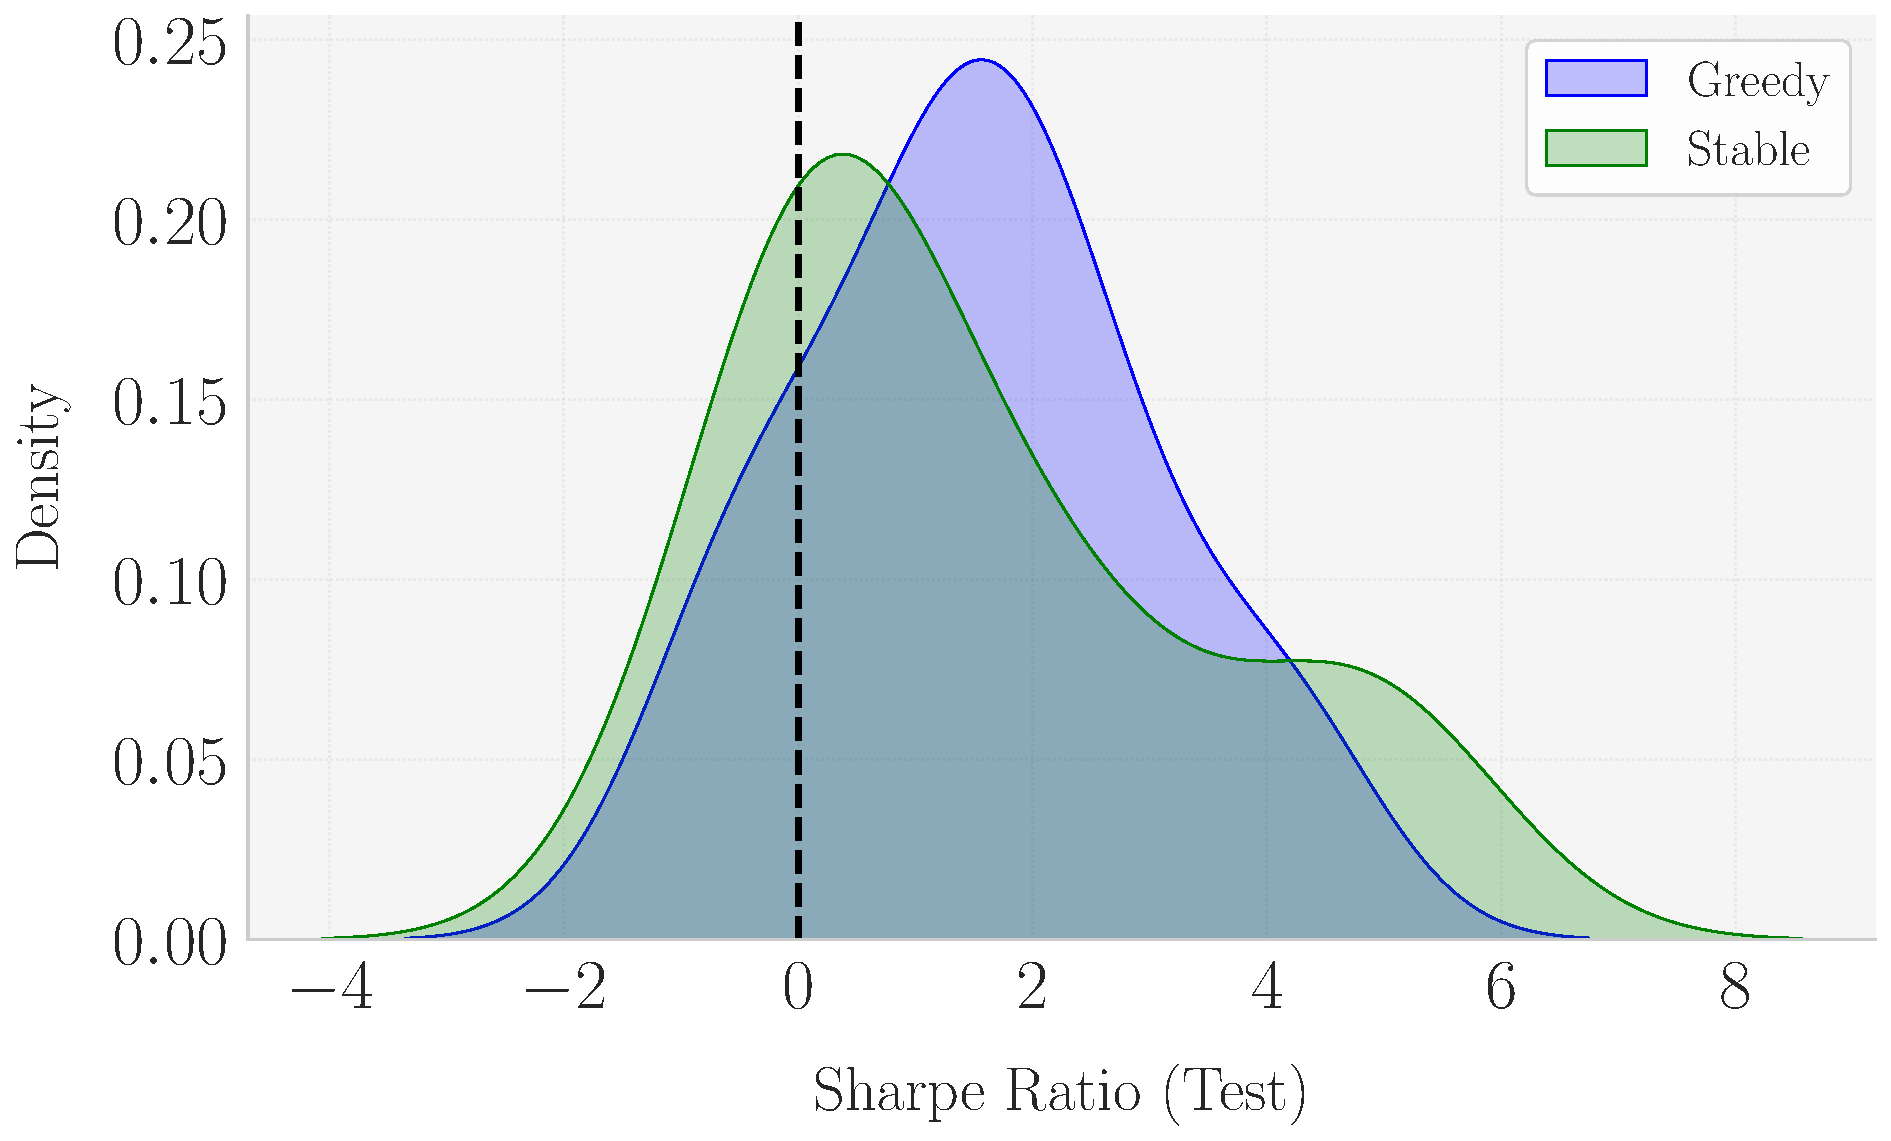
\includegraphics[width=\textwidth]{fig_8c_LLAMA_RobustnessCheck_SR_Test_Set_Distribution_[Change_L].pdf}
    \caption{\textbf{LLM}: Distribution of $SR^{\mathcal P^{test}}(L)$}
    \label{fig:LLM_Robustness_L_Distr}
  \end{subfigure}
  \hspace{0.05\textwidth} % Add horizontal space between the subfigures
  \begin{subfigure}[b]{0.44\textwidth}
    \centering
    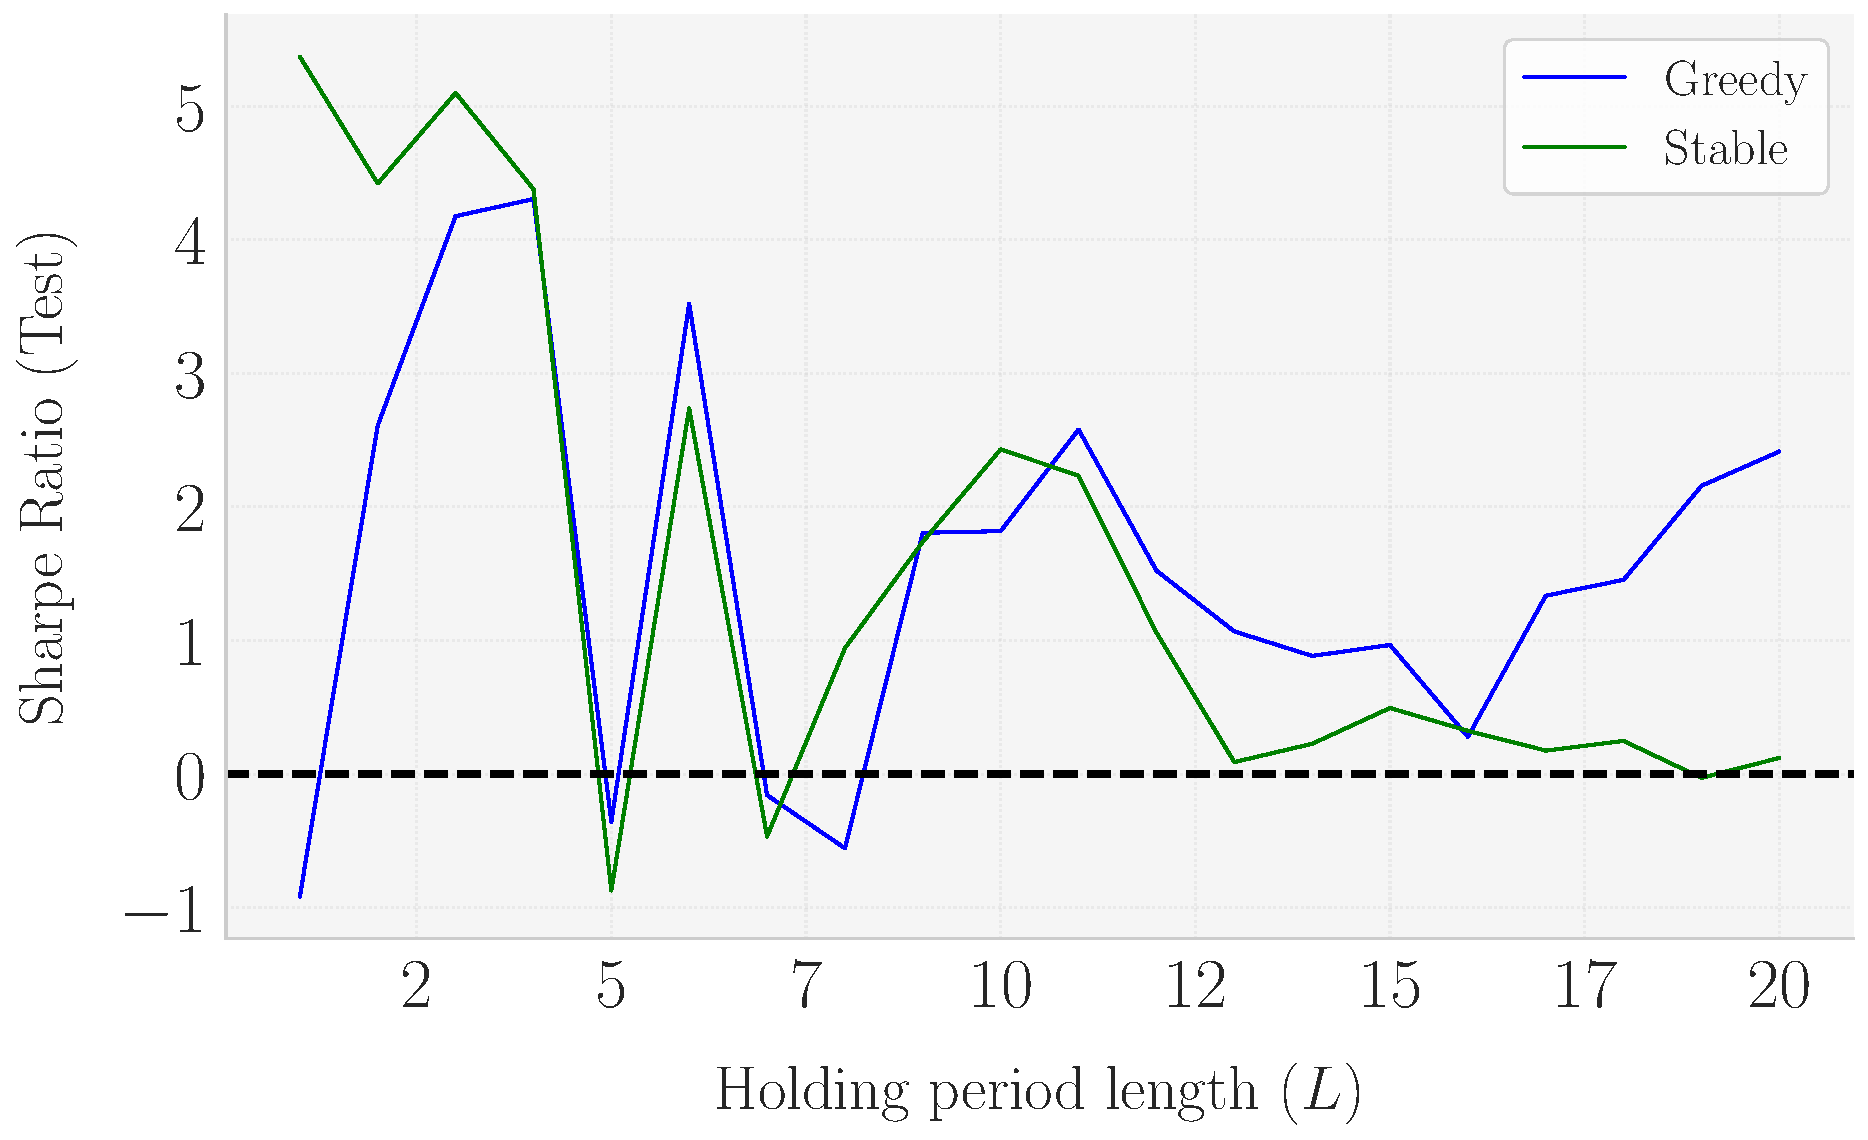
\includegraphics[width=\textwidth]{fig_8d_LLAMA_RobustnessCheck_SR_Test_Set_vs_L_[Change_L].pdf}
    \caption{\textbf{LLM}: Series of $SR^{\mathcal P^{test}}(L)$}
    \label{fig:LLM_Robustness_L_Series}
  \end{subfigure}
\label{fig:LLM_Robustness_L}
\mx 
\subcaption*{\textit{Note: This figure examines the sensitivity of the Sharpe Ratios ($SR^{\mathcal P^{test}}$) of the test portfolio to changes in the holding window length ($L$), with $\theta$ fixed at $\integer{0.5k}$. Panels \textsc{(a)} and \textsc{(b)} display the distribution and time series of $SR^{\mathcal P^{test}}(L)$ for KMeans clustering, respectively, while Panels \textsc{(c)} and \textsc{(d)} present the same for the LLM-based clustering. The left-hand panels show the skewness of the distributions: KMeans clustering results in a left-skewed distribution of Sharpe Ratios, whereas the LLM-based approach yields a right-skewed distribution, indicating higher profitability. The right-hand panels highlight that KMeans clustering only produces positive Sharpe Ratios for very short holding periods, whereas the LLM-based clustering shows more consistent positive performance across a wider range of $L$ values, though with some variability.}}
\end{figure}
%----------------------------------------------------

From \cref{fig:KMeans_Robustness_L_Distr} it follows that KMeans clustering produces a distribution that is clearly left-skewed, while the distribution of $SR^{\mathcal P ^{test}}$ for LLM clustering is clearly right-skewed (\cref{fig:LLM_Robustness_L_Distr}). This confirms the fact that LLM clustering generates Sharpe Ratios that are statistically higher than those generated by KMeans. The plots in the right-hand-side substantiate this observation: KMeans is only able to produce positive $SR^{\mathcal P ^{test}}$ for really short holding window lengths (\cref{fig:KMeans_Robustness_L_Series}), while LLM clustering, although not always stable, is, in general, able to produce positive Sharpe Ratios more consistently over the grid (\cref{fig:LLM_Robustness_L_Series}).

\mx 
We then turn to analyze the sensitivity of $SR^{\mathcal P^{test}}$ to different values for the upper bound on the number of traded clusters ($\theta$). Now we fix $L=4$ and define a grid $\b \theta$, from where we can obtain $\{SR^{\mathcal P^{test}}(\theta)\}_{\theta\in{\b\theta}}$. 


%----------------------------------------------------
\inserthere{fig:Robustness_theta}
\begin{figure}[H]
  \centering
  \caption{Sensitivity of $SR^{\mathcal P^{test}}$ to the upper bound on the number of traded clusters on each side ($\theta$)}
    \begin{subfigure}[b]{0.46\textwidth}
    \centering
    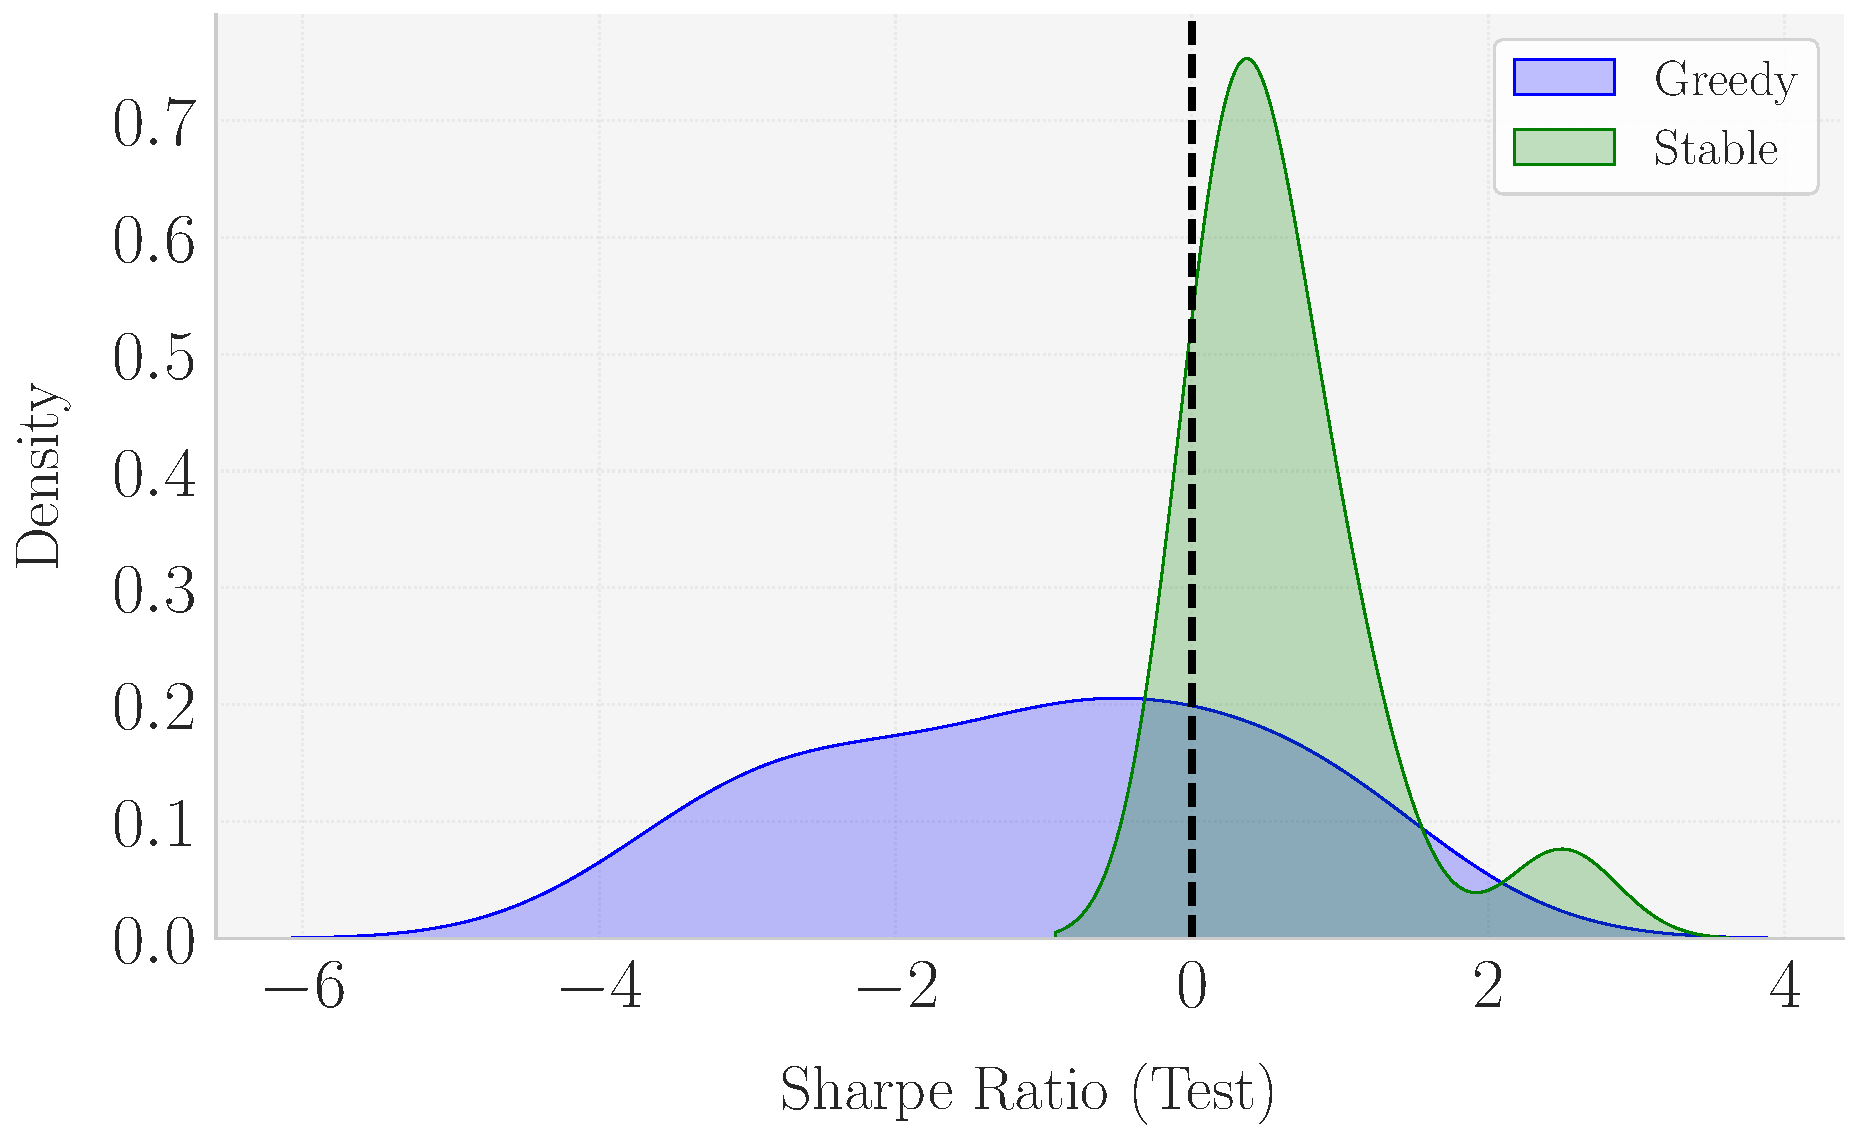
\includegraphics[width=\textwidth]{fig_9a_KMeans_RobustnessCheck_SR_Test_Set_Distribution_[Change_theta].pdf}
    \caption{\textbf{KMeans}: Distribution of $SR^{\mathcal P^{test}}(\theta)$}
    \label{fig:KMeans_Robustness_theta_Distr}
  \end{subfigure}
  \hspace{0.05\textwidth} % Add horizontal space between the subfigures
  \begin{subfigure}[b]{0.46\textwidth}
    \centering
    \includegraphics[width=\textwidth]{fig_9b_KMeans_RobustnessCheck_SR_Test_Set_vs_theta_[Change_theta].pdf}
    \caption{\textbf{KMeans}: Series of $SR^{\mathcal P^{test}}(\theta)$}
    \label{fig:KMeans_Robustness_theta_Series}
  \end{subfigure}
  
  \bx 
      \begin{subfigure}[b]{0.46\textwidth}
    \centering
    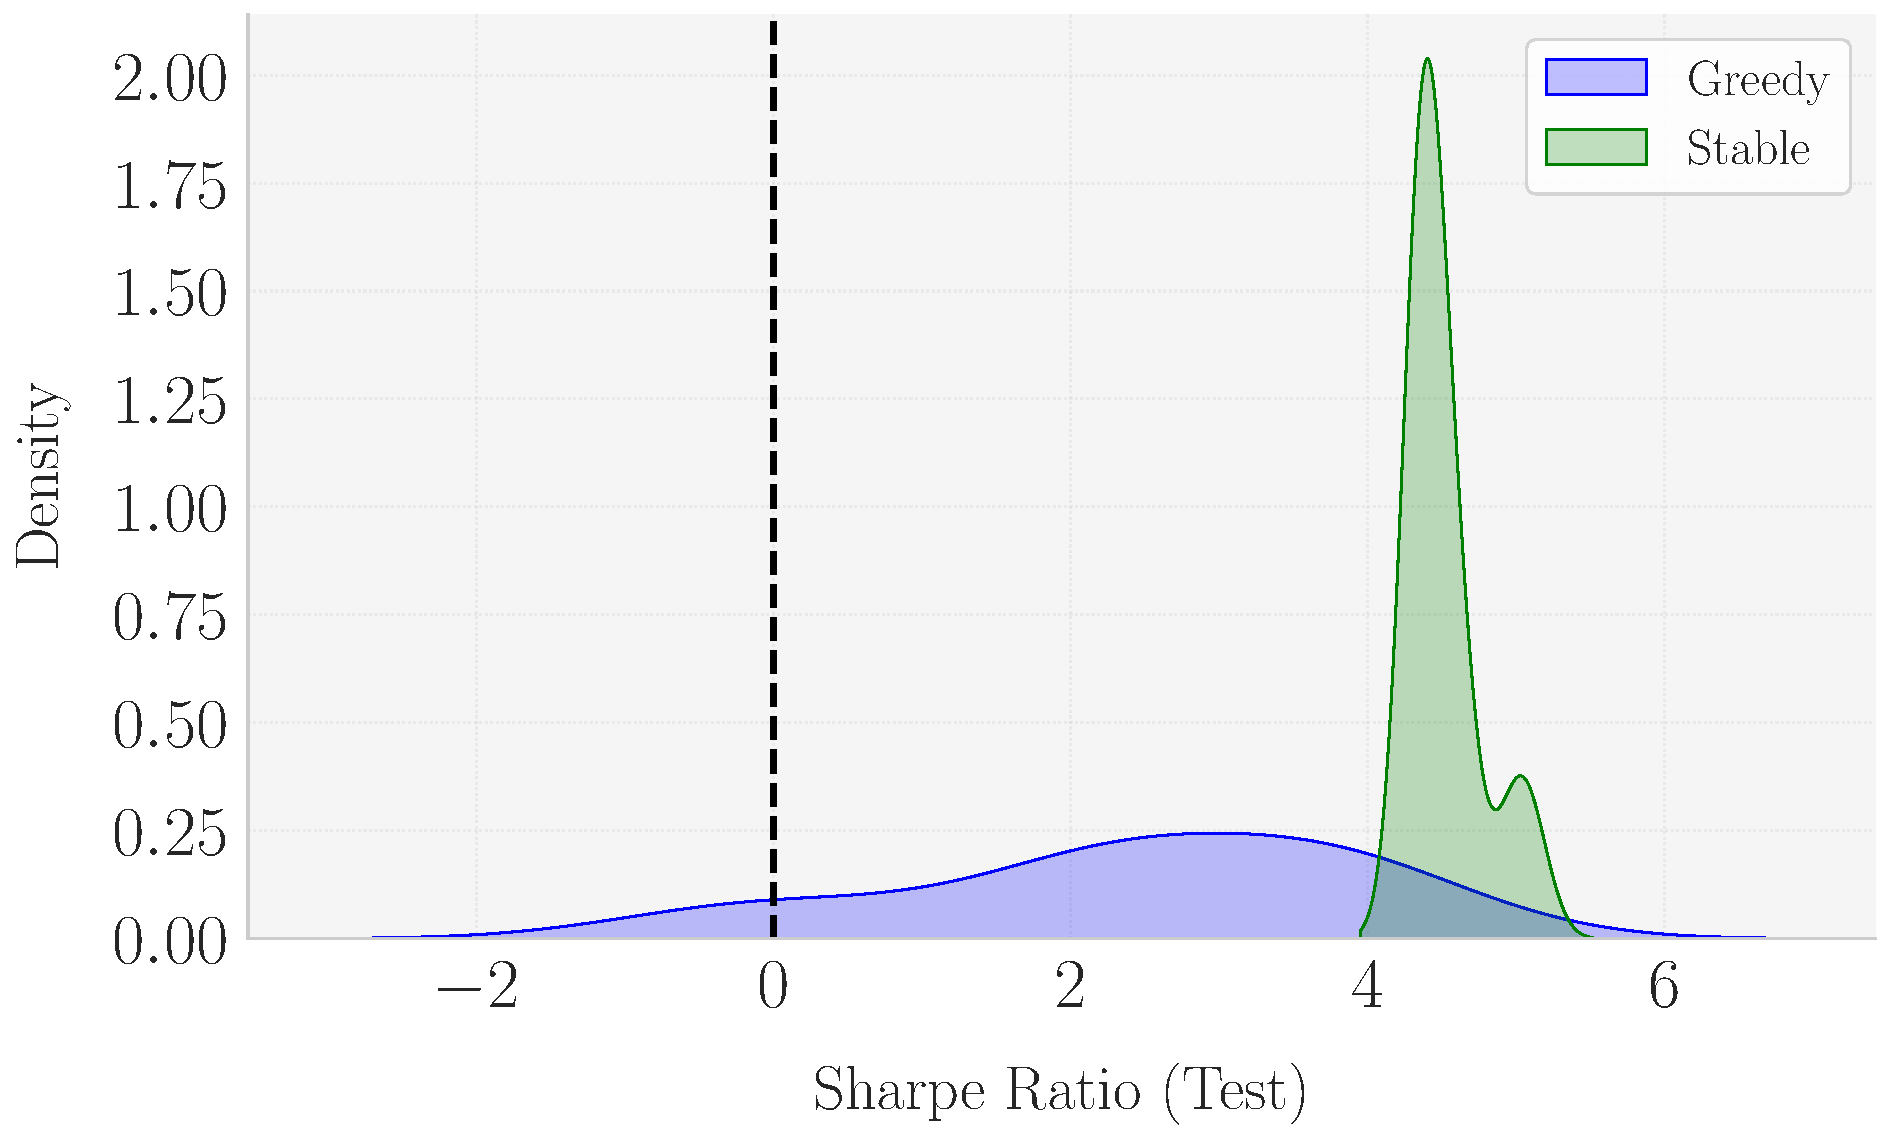
\includegraphics[width=\textwidth]{fig_9c_LLAMA_RobustnessCheck_SR_Test_Set_Distribution_[Change_theta].pdf}
    \caption{\textbf{LLM}: Distribution of $SR^{\mathcal P^{test}}(\theta)$}
    \label{fig:LLM_Robustness_theta_Distr}
  \end{subfigure}
  \hspace{0.05\textwidth} % Add horizontal space between the subfigures
  \begin{subfigure}[b]{0.46\textwidth}
    \centering
    \includegraphics[width=\textwidth]{fig_9d_LLAMA_RobustnessCheck_SR_Test_Set_vs_theta_[Change_theta].pdf}
    \caption{\textbf{LLM}: Series of $SR^{\mathcal P^{test}}(\theta)$}
    \label{fig:LLM_Robustness_theta_Series}
  \end{subfigure}

\mx 
\subcaption*{\textit{Note: This figure displays the sensitivity of the Sharpe Ratios ($SR^{\mathcal P^{test}}$) to variations in the upper bound on the number of traded clusters ($\theta$), with $L$ fixed at 4. Panels \textsc{(a)} and \textsc{(b)} show the distribution and series of $SR^{\mathcal P^{test}}(\theta)$ for KMeans clustering, respectively, while Panels \textsc{(c)} and \textsc{(d)} illustrate the same for LLM-based clustering. For KMeans, the results are mixed: the \textit{Stable} algorithm generates positive Sharpe Ratios for low $\theta$ values, whereas the \textit{Greedy} algorithm performs better with high $\theta$ values, indicating sensitivity and instability. In contrast, the LLM-based clustering shows a more consistent pattern, with a concentration of positive Sharpe Ratios across a broader range of $\theta$ values, suggesting greater robustness and stability in the trading strategy.}}

\label{fig:Robustness_theta}
\end{figure}
%----------------------------------------------------


The results of this exercise are shown in \cref{fig:Robustness_theta}. As we can see, in \cref{fig:KMeans_Robustness_theta_Distr} the results are mixed for the case of KMeans clustering. Namely, the \textit{Stable} algorithm is able to generate positive Sharpe Ratios but the \textit{Greedy} algorithm struggles to do so. In \cref{fig:KMeans_Robustness_theta_Series} we see what is happening: \textit{Stable} works well with for low values of $\theta$, while \textit{Greedy} only works for high values of $\theta$. This high reliance of the algorithms on specific values of $\theta$ points to the instability of the trading strategy when employing KMeans clustering.

\mx 
On the other hand, \cref{fig:LLM_Robustness_theta_Distr} shows a clear pattern for the case of LLM clustering. Namely, the mass accumulates at high and positive Sharpe Ratios. This observation is further substantiated by \cref{fig:KMeans_Robustness_theta_Series}, which shows that leaving aside the fact that the greedy algorithm does bad for really low values of $\theta$ (i.e.: $\theta\leq 3$), in general, the trading strategy is now able to produce high, positive and stable Sharpe Ratios across different values of $\theta$.  

\mx
All in all, our results are robust to hyperparameter variability, showing that LLM clustering consistently beats a strategy based on clustering embeddings with KMeans. 
